\section{Addressbar}
\subsection{Funktionen}
Die Addressbar prüft die Eingaben des Nutzers und schickt diese weiter an die WebView um die Seite anzeigen zu lassen.
Bei Eingabe einer URL wird diese geprüft und an die WebView weitergeschickt um die Webseite anzuzeigen.
Dabei wird die URL nur auf Vollständigkeit geprüft. Falls es dabei zu Fehlern kommt (fehlen von ''http://www'', ''http://'' oder ''www'')
wird die URL ergänzt und erst dann weitergeliefert.
Wenn es sich bei der Eingabe um keine URL handelt, wird die Eingabe an Google weitergeleitet und die Ergebnisse angezeigt.

\subsection{Implementierung}
Die in die Addressbar oder über den HomeButton eingegebene URL wird über die Funktion loadURL() an checkURL weitergeleitet.
Hier wird der String auf Fehler überprüft und der geänderte String zurückgegeben. Danach wird er mit loadRequest() an die
WebView weitergegeben.
\\\\
addressBar/homBTN():\\
Eingabe der URL als String.
\\\\
loadURL():\\
Aufrufe der Verarbeitungsschritte für die URL.
\\\\
checkURL():\\
Aufgeteilt in einzelne Funktinen, welche mit Hilfe von Regulären Ausdrücken die URL nach fehlenden Elementen prüfen.
Falls es Elemtent fehlt wird dieses hinzugefügt. Wenn es sich um keine URL handelt, wird eine URL für die Googlesuche erstellt.
\\\\
validateHTTPWWW():\\
Prüfen nach fehlendem ''http://www''.
\\
validateHTTP():\\
Prüfen nach fehlendem ''http://''.
\\
validateWWW():\\
Prüfen nach fehlendem ''www''.
\\\\
loadRequest:\\
Weitergabe der geprüften und verbesserten URL an die WebView.
\\\\
\begin{figure}
	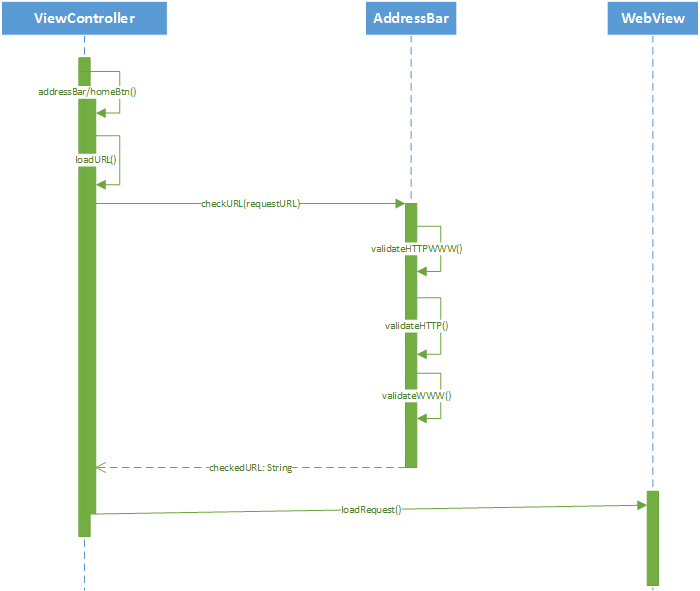
\includegraphics[width=\textwidth]{Pics/AddressCheck.png} 
	\caption{Sequenzdiagramm Adressbar}
	\label{fig:bild}
\end{figure}